\documentclass[CheatSheet]{subfiles}
\begin{document}


\summarystyle
\section{Kinematics}
\vspace{-1.5em}
\begin{lalignat*}{2}
\llabel{Notation here:}
p_i^\mu=\pmat{p^0_i\\\vc p_i},
\quad \tilde p_i=\norm{\vc p_i},
\quad E_i=\sqrt{\tilde p_i^2+m_i^2}\text{~(on-shell fixed)},
\quad Q_i=p_i^2=p^\mu_i p_{i \mu}.
\\&&&
\diracdeltabar[4]\left(P^\mu-p^\mu\right)\coloneq(2\pi)^4\diracdelta[4]\left(P^\mu-p^\mu\right)
\\&&&
\diracdeltabar\left((p^0)^2-E_p^2\right)\coloneq(2\pi)\diracdelta\left((p^0)^2-\vnorm{p}^2-m^2\right)\Theta\left(p^0\right)
\\&&&\text{K\"all\'en function}\quad
\Kallen(x,y,z) = x^2+y^2+z^2-2xy-2yz-2zx = (x-y-z)^2-4yz
\\&&&\text{LIPS}\quad
\dd\Pi = \ddP{p}\frac{1}{2E_{p}}
       = \frac{\dd p^0\dd^3\vc p}{(2\pi)^4}\diracdeltabar\left((p^0)^2-E_p^2\right)
\\&&&\phantom{\text{LIPS}}\quad
  \overline{\dd\Pi^{(n)}} \coloneq  {\dd\Pi_1\cdots\dd\Pi_n\,\diracdeltabar[4]\left(P^\mu-\sum p_n^\mu\right)}
\end{lalignat*}

\paragraph{Decay rate and cross section}  ($\mathcal M$ has a mass dimension of $4-N\w i-N\w f$.)
\begin{lalignat}{2}
\llabel{decay rate (rest frame; $\sqrt{s}=M_0$):}
\dd\Gamma=
\frac{1}{2M_0}\overline{\dd\Pi^{(N\w f)}}~
\Bigl|\mathcal M\left(M_0\to\left\{p_1, p_2,\cdots, p_{N\w f}\right\}\right)\Bigr|^2
\\
\llabel{cross section (Lorentz invariant):}
\dd\sigma =
\frac{1}{4E_AE_B\,v_{\text{M\o l}}}\overline{\dd\Pi^{(N\w f)}}~
\Bigl|\mathcal M\left(k_A,k_B\to\left\{p_1, p_2,\cdots, p_{N\w f}\right\}\right)\Bigr|^2
\\
\llabel{M\o ller parameter:}\notag
 4E_AE_B v_{\text{M\o l}}= 2s\cdot\Kallen[1/2](1,m_A^2/s,m_B^2/s).
\end{lalignat}


\paragraph{Mandelstam variables} For $(k_A,k_B)\to(p_1,p_2)$ collision,
\begin{alignat*}{3}
 &s = (k_A+k_B)^2 = (p_1+p_2)^2\qquad
 &&(k_A-k_B)^2 =  2(m_A^2+m_B^2)-s\qquad
 &&k_A\cdot k_B = (s-m_A^2-m_B^2)/2\\
 &t = (p_1-k_A)^2 = (p_2-k_B)^2
 &&(p_1-p_2)^2 = 2(m_1^2 + m_2^2) - s
 && p_1\cdot p_2 = (s-m_1^2-m_2^2)/2\\
 &u = (p_1-k_B)^2 = (p_2-k_A)^2
 &&&&k_A\cdot p_2 = (m_2^2 + m_A^2 - u)/2\\
 & s+t+u=m_A^2+m_B^2+m_1^2+m_2^2
 &&&&k_A\cdot p_1 = (m_1^2 + m_A^2 - t)/2
\end{alignat*}

\paragraph{Two-body final state in the CM frame}
$\displaystyle p_1^\mu+p_2^\mu=\pmat{E_1\\\vc p}+\pmat{E_2\\-\vc p}=\pmat{\sqrt s\\\vc 0}$
with $\vc p$ directing to $\Omega=(\theta,\phi)$:
\begin{align}
&\overline{\dd\Pi^{(2)}}\Big|\w{CM}
=\frac{\|\vc p\|}{4\pi\sqrt{s}}\frac{\dd\Omega}{4\pi}
=
\frac{\|\vc p\|}{8\pi \sqrt{s}}\dd\cos\theta
=
\frac{\Kallen[1/2](1,m_1^2/s,m_2^2/s)}{16\pi}\dd\cos\theta
\qquad \Bigl(\text{$\sqrt s = M_0$ or $E\w{CM}$}\Bigr)
\\
\notag&
\|\vc p\|=\frac{\sqrt{s}}{2}\Kallen[1/2]\left(1,\frac{m_1^2}{s},\frac{m_2^2}{s}\right),\quad
 E_1=\frac{s+m_1^2-m_2^2}{2\sqrt{s}},\quad
 E_2=\frac{s-m_1^2+m_2^2}{2\sqrt{s}},\quad
 p_1\cdot p_2 = \frac{s-(m_1^2+m_2^2)}{2}.
\end{align}
Decay rates and 2-to-2 cross sections are
\begin{align}
\dd\Gamma
&\stackrel{\text{CM}}{=}
\frac{\Kallen[1/2](1,m_1^2/s,m_2^2/s)}{32\pi M_0}
  \dd\cos\theta\,|\mathcal M|^2,
&
\dd\sigma
&\stackrel{\text{CM}}{=}
\frac{1}{32\pi s}
  \frac{\Kallen[1/2](1,m_1^2/s,m_2^2/s)}{\Kallen[1/2](1,m_A^2/s,m_B^2/s)}
  \dd\cos\theta\,|\mathcal M|^2
\end{align}


\begin{wrapfigure}[2]{r}{12em}\vspace{-1.5em}
 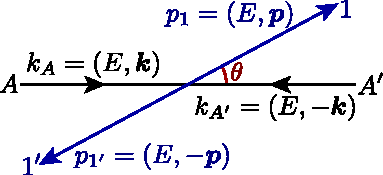
\includegraphics[width=\linewidth,page=1]{figs/collision.pdf}
\end{wrapfigure}

\noindent
For collisions with the same mass $(m_A,m_A)\to (m_1,m_1)$:
\begin{alignat*}{2}
t &= m_A^2+m_1^2 - s/2+2\tilde k\tilde p\cos\theta,\qquad
&\tilde k&={\sqrt{s/4-m_A^2}},\\
u &= m_A^2+m_1^2 - s/2-2\tilde k\tilde p\cos\theta,
&\tilde p&={\sqrt{s/4-m_1^2}}.
\end{alignat*}

\begin{wrapfigure}[2]{r}{12em}\vspace{-2em}
 \includegraphics[width=\linewidth,page=2]{figs/collision.pdf}
\end{wrapfigure}

\noindent
For collisions of massless initial particles $(0,0)\to (m_1,m_2)$:
\begin{alignat*}{2}
 t &= (m_1^2+m_2^2-s)/2+\tilde p\sqrt{s}\cos\theta,\qquad
&\tilde p&=(\sqrt{s}/2)\Kallen[1/2](1,m_1^2/s,m_2^2/s),\\
 u &= (m_1^2+m_2^2-s)/2-\tilde p\sqrt{s}\cos\theta.
\end{alignat*}

\paragraph{Phase-space reduction} With $Q'=p'^\mu p'_\mu$,
\begin{equation}
  \overline{\dd\Pi^{(n+m)}}(P;\,p_1,\dots,p_{n+m})
  =
  \overline{\dd\Pi^{(n)}}(p';\,p_1,\dots,p_n)\,
  \overline{\dd\Pi^{(m+1)}}(P;\,p',p_{n+1},\dots,p_{n+m})\frac{1}{2\pi}\dd Q'
  \label{eq:psreduction}
\end{equation}

\paragraph{Three-body final state} Mandelstam-like variables can be defined, for $P\to(p_1,p_2,p_3)$, as
\begin{equation*}
s_{ij}=(p_i+p_j)^2;\quad t_{0i}=(P-p_i)^2=s_{jk};\quad s_{12}+s_{23}+s_{31}=P^2+p_1^2+p_2^2+p_3^2.
\end{equation*}
For spherically-symmetric processes, the phase-space integral is reduced to, at the center-of-mass frame,
\begin{align}
\int\overline{\dd\Pi^3}_{\text{sph.\ sym.}}&(\sqrt{s}, \vc 0)
=\frac{1}{128\pi^3}\frac{1}{s}
\int_{(m_2+m_3)^2}^{(\sqrt{s}-m_1)^2}\dd s_{23}\int\dd s_{13};
\\ (s_{13})^{\text{max}}_{\text{min}} &=
\frac{(s+m_3^2-m_1^2-m_2^2)^2}{4s_{23}}
-\frac{1}{4s_{23}}
\left[\Kallen[1/2](s,m_1^2,s_{23})\mp\Kallen[1/2](s_{23},m_2^2,m_3^2)\right]^2
\notag\\&=(E_1^*+E_3^*)^2-\left(\sqrt{E_1^{*2}-m_1^2}\mp\sqrt{E_3^{*2}-m_3^2}\right)^2,
\quad
\end{align}
where 
$E_1^*=\frac{s-s_{23}-m_1^2}{2\sqrt{s_{23}}}$, and
$E_3^*=\frac{s_{23}-m_2^2+m_3^2}{2\sqrt{s_{23}}}$.

\newpage
\detailstyle
\subsection{Fundamentals}

Lorentz-invariant phase space:
\begin{align}
  \dd\Pi
   = \ddP{p}\frac{1}{2E_{p}}
   = \ddP{p}\frac{1}{2\sqrt{m^2+\tilde p^2}}
   = \frac{\dd p_0\dd^3\vc p}{(2\pi)^4}2\pi\diracdelta(p_0^2-\tilde p^2-m^2)\Theta(p^0)
   \equiv \frac{\dd p_0\dd^3\vc p}{(2\pi)^4}\diracdeltabar(p_0^2-E_p^2)
\end{align}
K\"all\'en function:
\begin{align*}
&\Kallen(x,y,z)
= x^2+y^2+z^2-2xy-2yz-2zx
= (x-y-z)^2-4yz;
\\
&
\Kallen(1;\alpha_1^2,\alpha_2^2)
= (1-(\alpha_1+\alpha_2)^2)(1-(\alpha_1-\alpha_2)^2)
= (1+\alpha_1+\alpha_2)(1-\alpha_1-\alpha_2)(1+\alpha_1-\alpha_2)(1-\alpha_1+\alpha_2).
\end{align*}
\begin{alignat*}{2}
&\Kallen[1/2]\left(s;m_1^2, m_2^2\right) = s\Kallen[1/2]\left(1;\frac{m_1^2}{s}, \frac{m_2^2}{s}\right);&
\qquad
&\Kallen[1/2]\left(1;\frac{m^2}{s},\frac{m^2}{s}\right)
= \sqrt{1-\frac{4 m^2}{s}},\\
&\Kallen[1/2]\left(1;\frac{m_1^2}{s},\frac{m_2^2}{s}\right)
= \sqrt{1-\frac{2 (m_1^2+m_2^2)}{s}+\frac{(m_1^2-m_2^2)^2}{s^2}},&
&\Kallen[1/2]\left(1;\frac{m_1^2}{s},0\right)
= \frac{s-m_1^2}{s}.
\end{alignat*}
\paragraph{Two-body phase space}
If $f(p_1^\mu,p_2^\mu)$ is Lorentz invariant, $f\equiv f(p_1^2,p_2^2,p_1^\mu p_{2\mu})\equiv f(\tilde p_1,\tilde p_2,\cos\theta_{12})$.
Meanwhile,
\begin{equation}
 \dd\Pi_1\dd\Pi_2
=
\ddP{p_1}\,\,\ddP{p_2}\frac{1}{2E_12E_2}
=
\frac{(4\pi)\dd\tilde p_1\,\tilde p_1^2}{(2\pi)^3}
\frac{(2\pi)\dd\tilde p_2\,\tilde p_2^2\,\dd\cos\theta_{12}}{(2\pi)^3}\frac{1}{2E_12E_2}
=
\frac{\dd E_+\dd E_- \dd s}{128\pi^4}
\end{equation}
with the replacement of the variables
\begin{align*}
& E_\pm = E_1\pm E_2,
\qquad
s=(p_1+p_2)^2=m_1^2 + m_2^2 + 2E_1E_2 - 2\tilde p_1 \tilde p_2\cos\theta_{12};\\
&
\left|\frac{\dd(E_+,E_-,s)}{\dd(\tilde p_1,\tilde  p_2, \cos\theta_{12})}\right|=\frac{4\tilde p_1^2\tilde p_2^2}{E_1E_2},
\qquad
\left|\frac{\dd(E_1,E_2,s)}{\dd(\tilde p_1,\tilde  p_2, \cos\theta_{12})}\right|=\frac{2\tilde p_1^2\tilde p_2^2}{E_1E_2}.
\end{align*}
Therefore, 
\begin{equation}
 \int\dd\Pi_1\dd\Pi_2
=
\frac{1}{128\pi^4}
\int_{(m_1+m_2)^2}^\infty\dd s
\int_{\sqrt{s}}^\infty\dd E_+
\int\w{min}^{\mathrm{max}}\dd E_-,
\end{equation}
where the boundary of $E_-$ is given by
\begin{align*}
 &\cos\theta_{12}=\frac{E_+^2-E_-^2+2 \left(m_1^2+m_2^2-s\right)}{\sqrt{(E_++E_-)^2-4 m_1^2}\sqrt{(E_+-E_-)^2-4 m_2^2}} \in [-1,1]\\
 &\therefore\quad
\left|E_- - \frac{m_1^2-m_2^2}{s}E_+\right| 
\le
\sqrt{E_+^2-s}\cdot\Kallen[1/2]\left(1;\frac{m_1^2}{s},\frac{m_2^2}{s}\right).
\end{align*}

\paragraph{Two-body phase space with momentum conservation}
We consider general two-body phase-space integrals,
\begin{equation}
 \overline{\dd\Pi^{(2)}}\times I
   = \dd\Pi_1\dd\Pi_2\,\diracdeltabar[4](P^\mu-p_1^\mu-p_2^\mu)\times I
   =\frac{1}{(2\pi)^2}\frac{\dd^3{\vc p_1}}{2E_1}\frac{\dd^3{\vc p_2}}{2E_2}\diracdelta[4](P^\mu-p_1^\mu-p_2^\mu)\times I
\end{equation}
with $I$ being the integrand, $P^\mu=(E_0, \vc P_0)$, and $S_0=E_0^2-\tilde P_0^2$, assuming $S_0>0$. First, with carrying out $\vc p_2$ integral,

\begin{align}
 \overline{\dd\Pi^{(2)}}\times I
  &= \frac{1}{(2\pi)^2}\frac{\dd^3{\vc p_1}}{2E_1}{\dd^4 p_2^\mu}
  \diracdelta((p_2^0)^2-\|\vc p_2\|^2-m_2^2)\Theta(p_2^0)
  \diracdelta[4](P^\mu-p_1^\mu-p_2^\mu)\times I
  \\&=
   \frac{1}{(2\pi)^2}\frac{\dd^3{\vc p_1}}{2E_1}
  \diracdelta((E_0-E_1)^2-\|\vc P_0-\vc p_1\|^2-m_2^2)\Theta(E_0-E_1)\times I
  \\&=
   \frac{1}{(2\pi)^2}\frac{\dd^3{\vc p_1}}{2E_1}
  \diracdelta(S_0-2E_0E_1+2\vc P_0\cdot\vc p_1+m_1^2-m_2^2)\Theta(E_0-E_1)\times I
  \\&=
   \frac{\tilde p_1\dd E_1\dd\cos\theta\dd\phi}{8\pi^2}
  \diracdelta(S_0-2E_0E_1+2\tilde P_0\tilde p_1\cos\theta+m_1^2-m_2^2)\Theta(E_0-E_1)\times I~\Big|_{\tilde p_1=(E_1^2-m_1^2)^{1/2}}.
\end{align}


Now, we continue for a constant $I$.  If $\tilde P_0=0$, then $\sqrt {S_0}=E_0$ and
\begin{equation}
 \overline{\dd\Pi^{(2)}}
  =
   \frac{(E_1^2-m_1^2)^{1/2}\dd E_1}{2\pi}
  \diracdelta(2\sqrt{S_0}\mathcal E-2E_0E_1)\Theta(E_0-E_1)
  =
   \frac{\phi}{4\pi\sqrt{S_0}}
\end{equation}
to recover the CM result with the constants
\begin{equation}
  \mathcal E=\frac{S_0+m_1^2-m_2^2}{2\sqrt{S_0}},\qquad
  \phi=\frac{\Kallen[1/2](S_0,m_1^2,m_2^2)}{2\sqrt{S_0}}=\sqrt{\mathcal E^2-m_1^2}.
\end{equation}

Because the result is Lorentz scalar, the result is unchanged even if $\tilde P_0\neq 0$ as we explicitly check by integrating $\cos\theta$; the integration gives the Heaviside function and
\begin{align}
 \overline{\dd\Pi^{(2)}}
&=
   \frac{1}{8\pi\tilde P_0}\int_{m_1}^{E_0}{\dd E_1}\,
  \Theta\left(-1<c(E_1)<1\right);\qquad
  c(E_1)\coloneq \frac{E_0E_1-\sqrt{S_0}\mathcal E}{\tilde P_0(E_1^2-m_1^2)^{1/2}}.
\end{align}
There,
\begin{align}
  &E_{\text{1; max}}=\frac{E_0\mathcal E+\tilde P_0\phi}{\sqrt {S_0}}
  \quad\iff\quad
\tilde p_1=\frac{\tilde P_0\mathcal E+E_0\phi}{\sqrt{S_0}}
  \quad\then c=+1,
\\&
  E_{\text{1; min}}=\frac{E_0\mathcal E-\tilde P_0\phi}{\sqrt {S_0}}
  \quad\iff\quad
\tilde p_1=\left|\frac{\tilde P_0\mathcal E-E_0\phi}{\sqrt{S_0}}\right|
  \quad\then c = \sign(\tilde P_0\mathcal E-E_0\phi).
\end{align}
If $\tilde P_0\mathcal E-E_0\phi<0$, the first derivative $c'(E_1)$ cannot be zero between $E_{\text{1; min}}$ and $E_{\text{1; max}}$, so $c(E_1)$ is monotonically increasing and $E_1$ and $\cos\theta$ are in one-to-one correspondence. Meanwhile, if $\tilde P_0\mathcal E-E_0\phi>0$, then $c(E_1)$ has a minimum
\begin{equation}
  c\w{min}=c\left(\frac{E_0m_1^2}{S_0\mathcal E}\right)
  = \frac{\sqrt{E_0^2 m_1^2-S \mathcal E^2}}{\tilde P_0 m_1}=\sqrt{1-\frac{S \phi ^2}{m_1^2\tilde P_0^2}}.
\end{equation}
In any cases, all $E_1$ between them are allowed, and we evaluate $\overline{\dd\Pi^{(2)}}
=
   (E_{\text{1; max}}-E_{\text{1; min}})/8\pi\tilde P_0=\phi/4\pi\sqrt{S_0}$ as expected.


\subsection{Decay rate and Cross section}
As
$\braket{\text{out}|\text{in}}=(2\pi)^4\diracdelta[4](p\w i-p\w f)\ii\mathcal M$
(for $\text{in}\neq\text{out}$) and $\braket{\vc p|\vc p}=2E_{\vc p}(2\pi)^3\diracdelta[3](\vc 0)=2E_\vc {p}V$ for one-particle state,
\begin{equation}
 \frac{N\w{ev}}{\prod\w{in} N\w{particle}}
= \int\dd\Pi^{\mathrm{out}}\frac{\left|\braket{\text{out}|\text{in}}\right|^2}{\braket{\text{in}|\text{in}}}
= \int\dd\Pi^{\mathrm{out}}\frac{(2\pi)^8|\mathcal M|^2}{\prod\w{in}(2E)V}
\frac{VT}{(2\pi)^4}\diracdelta[4](p\w i-p\w f)
  = VT\int\overline{\dd\Pi^{(N\w f)}}\frac{|\mathcal M|^2}{\prod\w{in}(2E)V}.
\end{equation}
Therefore, decay rate (at the rest frame) is given by
\begin{equation}
 \dd\Gamma
\coloneq  \frac{1}{T}\frac{\dd N\w{ev}}{N\w{particle}}
 = \frac{1}{T}VT\overline{\dd\Pi^{(N\w f)}}\frac{|\mathcal M|^2}{(2E)V}
 = \frac{1}{2M_0}\overline{\dd\Pi^{(N\w f)}}{|\mathcal M|^2}.
\end{equation}
We also define Lorentz-invariant cross section $\sigma$ by $N\w{ev}\eqcolon(n_A v_{\text{M\o l}}T\sigma)N_B=(n_A v_{\text{M\o l}}T\sigma)(n_B V)$ with
number density $n$, or
\begin{equation}
\dd\sigma\coloneq \frac{\dd N\w{ev}}{n_A v_{\text{M\o l}}TN_B}
=
\frac{V}{v_{\text{M\o l}}T}
VT\overline{\dd\Pi^{(N\w f)}}\frac{|\mathcal M|^2}{2E_A2E_BV^2}
=
\frac{1}{2E_A2E_B\,v_{\text{M\o l}}}
\overline{\dd\Pi^{(N\w f)}}|\mathcal M|^2,
\end{equation}
where the M\o ller parameter $v_{\text{M\o l}}$ is equal to $v^{\mathrm{NR}}\w{rel}=\|\vc v_A-\vc v_B\|$ if $\vc v_A\parallel\vc v_B$ (cf.~Ref.~\cite{Cannoni:2016hro}).
Generally,
\begin{equation}
  v_{\text{M\o l}}\coloneq 
 \frac{\sqrt{(p_A\cdot p_B)^2-m_A^2m_B^2}}{E_AE_B}
=\frac{\sqrt{\Kallen(s,m_A^2,m_B^2)}}{2E_AE_B}
=\frac{p_A\cdot p_B}{E_A E_B}v\w{rel}
=({1-\vc v_A\cdot\vc v_B})v\w{rel},
\end{equation}
where $v\w{rel}$ is the actual relative velocity
\begin{equation}
  v\w{rel}
=\sqrt{1-\frac{(1-v_A^2)(1-v_B^2)}{1-(\vc v_A\cdot\vc v_B)^2}}
=\frac{\sqrt{\|\vc v_A-\vc v_B\|^2-\|\vc v_A\times\vc v_B\|^2}}{1-\vc v_A\cdot\vc v_B} =\frac{\Kallen[1/2](s,m_A^2,m_B^2)}{s-(m_A^2+m_B^2)}\neq v^{\mathrm{NR}}\w{rel}.
\end{equation}
(Note that $p_A\cdot p_B/E_AE_B=1$ if $\vc p_A=0$ or $\vc p_B=0$. Also, Each of $v\w{rel}$, $VT$, and $E_AE_Bv_{\text{M\o l}}$ is Lorentz invariant.)



\subsection{More than two bodies}
The phase-space reduction formula \eqref{eq:psreduction} is proved by, with $p_{a,\dots,b}=\sum_{i=a}^b p_i$, (cf.~Ref.~\cite{Hitoshi233B})
\begin{align*}
  \overline{\dd\Pi^{(n+m)}}%(P;\,p_1,\dots,p_{n+m})
  &=\left[
    \ddP{p'}\frac{\dd p'^0}{2\pi}\diracdeltabar[4]\left(p'^\mu-p_{1,\dots,n}^\mu\right)
  \right]
  \dd\Pi_1\cdots\dd\Pi_{n+m}\,\diracdeltabar[4]\left(P^\mu-p_{1,\dots,n+m}^\mu\right)
\\ &=    \left[
    \overline{\dd\Pi^{(n)}}(p';\,p_1,\dots,p_n)\,
    \overline{\dd\Pi^{(m+1)}}(P;\,p',p_{n+1},\dots,p_{n+m})\,
  \right]
    \frac{\dd p'^0}{2\pi}(2p'^0)
\\ &=    \left[
    \overline{\dd\Pi^{(n)}}(p';\,p_1,\dots,p_n)\,
    \overline{\dd\Pi^{(m+1)}}(P;\,p',p_{n+1},\dots,p_{n+m})\,
  \right]_{p'^\mu p'_\mu=Q'\text{~:~fixed}}
    \frac{\dd Q'}{2\pi}.
\end{align*}

\pagebreak[3]

The phase-space integral of massless $n$-body particles over a constant is obtained by, as we can set $P^\mu=\spmat{\sqrt{s}\\\vc 0}$,
\begin{align}
\int1\,\overline{\dd\Pi^{(n)}}(s)
&= \frac{\dd Q'}{2\pi}
  \overline{\dd\Pi^{(2)}}(P;\,p',p_{n})\,
  \overline{\dd\Pi^{(n-1)}}(p';\,p_1,\dots,p_{n-1})
\notag\\&= \frac{\dd Q'}{2\pi}
  \frac{\tilde p'}{4\pi P^0}
  a_{n-1}Q'^{n-3}
= \frac{\dd Q'}{2\pi}
  \frac{s-Q'}{8\pi{s}}
  a_{n-1}Q'^{n-3}
= \frac{a_{n-1}}{(4\pi)^2(n-1)(n-2)}s^{n-2}
\notag\\&\therefore\quad
\int1\,\overline{\dd\Pi^{(n)}}=
  \frac{1}{2(4\pi)^{2n-3}}\frac{s^{n-2}}{(n-1)!(n-2)!}
\end{align}
where the fact is used that $\overline{\dd\Pi^{(n)}}(s)=a_n\times s^{n-2}$ with $a_n$ being a constant.


\paragraph{Three-body: spherically-symmetric cases}
The three-body phase space integral is reduced as
\begin{align}
  &\overline{\dd\Pi^{(3)}}
  =\frac{\dd Q_{23}}{2\pi}
  \overline{\dd\Pi^{(2)}}(P;\,p_1,p_{23})
  \overline{\dd\Pi^{(2)}}(p_{23};\,p_2,p_3),
\\&
\qquad\overline{\dd\Pi^{(2)}}(p_{23};\,p_2,p_3)=
\frac{\dd\cos\theta_{2}}{8\pi}
\frac{\tilde p_{2}^2}{E_{23}\tilde p_2 - \tilde p_{23}E_2\cos\theta_2};
\\
&
\qquad\tilde p_2=\frac{(Q_{23}+m_2^2-m_3^2)\tilde p_{23}\cos\theta_2
 + E_{23}\sqrt{\Kallen(Q_{23},m_2^2,m_3^2)-4m_2^2\tilde p_{23}^2 \sin^2\theta_2}
}{2(Q_{23}+\tilde p_{23}^2\sin^2\theta_2)},
\end{align}
where $\theta_2$ is the angle between $\vc p_{23}$ and $\vc p_2$ (in the lab frame).
If the matrix element to integrate is spherically symmetric, so as $\overline{\dd\Pi^{(2)}}(p_{23};p_2,p_3)|\mathcal M|^2$, i.e., it is independent of the angle of $\vc p_{23}$. Then one can simply evaluate  $\int\dd^3\vc p_{23}$, which leads to, in the center-of-mass frame,
\begin{equation}
\overline{\dd\Pi^3}_{\text{sph.\ sym.}}(\sqrt{s}, \vc 0)
=
\frac{\dd s_{23}\dd\cos\theta_{2}}{64\pi^3}
\frac{p_1}{\sqrt s}
\frac{p_{2}^2}{p_2\sqrt{s_{23}+p_1^2} - p_1\sqrt{p_2^2+m_2^2}\cos\theta_2}\Big|_{
 p_1^2=\lambda(s,m_1^2,s_{23})/4s
}
= \frac{s}{128\pi^3}\dd x_1\dd x_2,
\end{equation}
where we defined $x_i\coloneq {2E_i}/{\sqrt s}$. Noting that $s_{23}=s+m_1^2-2E_1\sqrt{s}=s(1-x_1)+m_1^2$ etc., 
\begin{equation}
 \overline{\dd\Pi^3}_{\text{sph.\ sym.}}(\sqrt{s}, \vc 0)
=
\frac{1}{128\pi^3}\frac{1}{s}
\int_{(m_2+m_3)^2}^{(\sqrt{s}-m_1)^2}\dd s_{23}\int\dd s_{13};
\end{equation}
\begin{equation}
 (s_{13})^{\text{max}}_{\text{min}} =
\frac{(s+m_3^2-m_1^2-m_2^2)^2}{4s_{23}}
-\frac{1}{4s_{23}}
\left[\Kallen[1/2](s,m_1^2,s_{23})\mp\Kallen[1/2](s_{23},m_2^2,m_3^2)\right]^2.
\end{equation}
This is equal to the PDG-Eq.~(47.23)\cite{PDG2018}.


\subsection{Two-body decay of boosted particles}
A particle with $(P, \Theta, \Phi; M)$ decaying to two particles; at the CM frame the momenta of the decay products are characterized by $\vc q=(q,\theta,\phi)$ with $q=(M_0/2)\Kallen[1/2](1,m_1^2/M_0^2,m_2^2/M_0^2)$. Their lab-frame momenta are given by
\begin{align}
 P &=
\begin{pmatrix}
  E_0\\
 {P_0} \si\Theta \co\Phi \\
 {P_0} \si\Theta \si\Phi \\
 {P_0} \co\Theta \\
\end{pmatrix},&
 p_1&=
\begin{pmatrix}
  ({E_0 \mathcal{E}_1+P_0 q \co\theta})/{M_0} \\
 q \co\Theta \co\Phi \si\theta \co\phi - q \si\Phi \si\theta \si\phi + r_1 \si\Theta \co\Phi \\
 q \co\Theta \si\Phi \si\theta \co\phi + q \co\Phi \si\theta \si\phi   + r_1 \si\Theta \si\Phi \\
 -q \si\Theta \si\theta \co\phi + r_1 \co\Theta\\
\end{pmatrix},&
p_2&=
\begin{pmatrix}
  ({E_0 \mathcal{E}_2-P_0 q \co\theta})/{M_0} \\
 -q \co\Theta \co\Phi \si\theta \co\phi + q \si\Phi \si\theta \si\phi + r_2 \si\Theta \co\Phi \\
 -q \co\Theta \si\Phi \si\theta \co\phi - q \co\Phi \si\theta \si\phi + r_2 \si\Theta\si\Phi  \\
  q \si\Theta \si\theta \co\phi+r_2 \co\Theta \\
\end{pmatrix}
\end{align}
with $r_1=(P_0\mathcal{E}_1+E_0q\co\theta)/M_0$, $r_2=(P_0\mathcal{E}_2-E_0q\co\theta)$, and $\mathcal{E}_i=\sqrt{m_i^2+q^2}$.


\end{document}
